\documentclass{article}\usepackage[]{graphicx}\usepackage[]{color}
%% maxwidth is the original width if it is less than linewidth
%% otherwise use linewidth (to make sure the graphics do not exceed the margin)
\makeatletter
\def\maxwidth{ %
  \ifdim\Gin@nat@width>\linewidth
    \linewidth
  \else
    \Gin@nat@width
  \fi
}
\makeatother

\definecolor{fgcolor}{rgb}{0.345, 0.345, 0.345}
\newcommand{\hlnum}[1]{\textcolor[rgb]{0.686,0.059,0.569}{#1}}%
\newcommand{\hlstr}[1]{\textcolor[rgb]{0.192,0.494,0.8}{#1}}%
\newcommand{\hlcom}[1]{\textcolor[rgb]{0.678,0.584,0.686}{\textit{#1}}}%
\newcommand{\hlopt}[1]{\textcolor[rgb]{0,0,0}{#1}}%
\newcommand{\hlstd}[1]{\textcolor[rgb]{0.345,0.345,0.345}{#1}}%
\newcommand{\hlkwa}[1]{\textcolor[rgb]{0.161,0.373,0.58}{\textbf{#1}}}%
\newcommand{\hlkwb}[1]{\textcolor[rgb]{0.69,0.353,0.396}{#1}}%
\newcommand{\hlkwc}[1]{\textcolor[rgb]{0.333,0.667,0.333}{#1}}%
\newcommand{\hlkwd}[1]{\textcolor[rgb]{0.737,0.353,0.396}{\textbf{#1}}}%
\let\hlipl\hlkwb

\usepackage{framed}
\makeatletter
\newenvironment{kframe}{%
 \def\at@end@of@kframe{}%
 \ifinner\ifhmode%
  \def\at@end@of@kframe{\end{minipage}}%
  \begin{minipage}{\columnwidth}%
 \fi\fi%
 \def\FrameCommand##1{\hskip\@totalleftmargin \hskip-\fboxsep
 \colorbox{shadecolor}{##1}\hskip-\fboxsep
     % There is no \\@totalrightmargin, so:
     \hskip-\linewidth \hskip-\@totalleftmargin \hskip\columnwidth}%
 \MakeFramed {\advance\hsize-\width
   \@totalleftmargin\z@ \linewidth\hsize
   \@setminipage}}%
 {\par\unskip\endMakeFramed%
 \at@end@of@kframe}
\makeatother

\definecolor{shadecolor}{rgb}{.97, .97, .97}
\definecolor{messagecolor}{rgb}{0, 0, 0}
\definecolor{warningcolor}{rgb}{1, 0, 1}
\definecolor{errorcolor}{rgb}{1, 0, 0}
\newenvironment{knitrout}{}{} % an empty environment to be redefined in TeX

\usepackage{alltt}

\usepackage{booktabs}

\usepackage{wasysym}
\renewcommand{\familydefault}{\sfdefault}
\IfFileExists{upquote.sty}{\usepackage{upquote}}{}
\begin{document}

\begin{knitrout}
\definecolor{shadecolor}{rgb}{0.969, 0.969, 0.969}\color{fgcolor}\begin{kframe}


{\ttfamily\noindent\color{warningcolor}{\#\# Warning in readChar(con, 5L, useBytes = TRUE): cannot open compressed file 'EnvSelFluA.RData', probable reason 'No such file or directory'}}

{\ttfamily\noindent\bfseries\color{errorcolor}{\#\# Error in readChar(con, 5L, useBytes = TRUE): cannot open the connection}}

{\ttfamily\noindent\color{warningcolor}{\#\# Warning in readChar(con, 5L, useBytes = TRUE): cannot open compressed file 'EnvQGA.RData', probable reason 'No such file or directory'}}

{\ttfamily\noindent\bfseries\color{errorcolor}{\#\# Error in readChar(con, 5L, useBytes = TRUE): cannot open the connection}}

{\ttfamily\noindent\bfseries\color{errorcolor}{\#\# Error in library(xtable): there is no package called 'xtable'}}

{\ttfamily\noindent\bfseries\color{errorcolor}{\#\# Error in library(MCMCglmm): there is no package called 'MCMCglmm'}}\end{kframe}
\end{knitrout}




\begin{knitrout}
\definecolor{shadecolor}{rgb}{0.969, 0.969, 0.969}\color{fgcolor}\begin{kframe}
\begin{alltt}
\hlkwd{setPar}\hlstd{()}
\hlkwd{plot}\hlstd{(SelAByYear,} \hlkwc{x}\hlstd{=}\hlnum{2006}\hlopt{:}\hlnum{2015}\hlstd{,} \hlkwc{ylim}\hlstd{=}\hlkwd{c}\hlstd{(}\hlkwd{min}\hlstd{( CISelAByYear),} \hlkwd{max}\hlstd{( CISelAByYear)),} \hlkwc{xlab}\hlstd{=}\hlstr{"Year"}\hlstd{,} \hlkwc{ylab} \hlstd{=} \hlstr{"Selection gradient"}\hlstd{,} \hlkwc{main} \hlstd{=} \hlstr{"\textbackslash{}\textbackslash{}textbf\{(A)\} Total selection"}\hlstd{)}
\end{alltt}


{\ttfamily\noindent\bfseries\color{errorcolor}{\#\# Error in xy.coords(x, y, xlabel, ylabel, log): object 'SelAByYear' not found}}\begin{alltt}
\hlkwd{abline}\hlstd{(}\hlkwc{h}\hlstd{=}\hlnum{0}\hlstd{)}
\end{alltt}


{\ttfamily\noindent\bfseries\color{errorcolor}{\#\# Error in int\_abline(a = a, b = b, h = h, v = v, untf = untf, ...): plot.new has not been called yet}}\begin{alltt}
\hlkwd{arrows}\hlstd{(}\hlkwc{x0} \hlstd{=} \hlnum{2006}\hlopt{:}\hlnum{2015}\hlstd{,}\hlkwc{x1} \hlstd{=} \hlnum{2006}\hlopt{:}\hlnum{2015}\hlstd{,}\hlkwc{code} \hlstd{=} \hlnum{3}\hlstd{,} \hlkwc{y0} \hlstd{= CISelAByYear[}\hlnum{1}\hlstd{,],}
       \hlkwc{y1} \hlstd{= CISelAByYear[}\hlnum{2}\hlstd{,],} \hlkwc{angle} \hlstd{=} \hlnum{90}\hlstd{,}\hlkwc{length} \hlstd{=} \hlnum{0.1}\hlstd{)}
\end{alltt}


{\ttfamily\noindent\bfseries\color{errorcolor}{\#\# Error in arrows(x0 = 2006:2015, x1 = 2006:2015, code = 3, y0 = CISelAByYear[1, : object 'CISelAByYear' not found}}\begin{alltt}
\hlkwd{abline}\hlstd{(}\hlkwc{h}\hlstd{=}\hlkwd{coefficients}\hlstd{(m0all)[}\hlnum{2}\hlstd{],} \hlkwc{lty}\hlstd{=}\hlnum{2}\hlstd{,} \hlkwc{lwd}\hlstd{=}\hlnum{5}\hlstd{)}
\end{alltt}


{\ttfamily\noindent\bfseries\color{errorcolor}{\#\# Error in coefficients(m0all): object 'm0all' not found}}\begin{alltt}
\hlstd{lowm0all} \hlkwb{<-} \hlkwd{coefficients}\hlstd{(m0all)[}\hlnum{2}\hlstd{]}\hlopt{+}\hlnum{1.96}\hlopt{*}\hlstd{sm0all}\hlopt{$}\hlstd{coefficients[}\hlnum{2}\hlstd{,}\hlnum{2}\hlstd{]}
\end{alltt}


{\ttfamily\noindent\bfseries\color{errorcolor}{\#\# Error in coefficients(m0all): object 'm0all' not found}}\begin{alltt}
\hlstd{highm0all} \hlkwb{<-} \hlkwd{coefficients}\hlstd{(m0all)[}\hlnum{2}\hlstd{]}\hlopt{-}\hlnum{1.96}\hlopt{*}\hlstd{sm0all}\hlopt{$}\hlstd{coefficients[}\hlnum{2}\hlstd{,}\hlnum{2}\hlstd{]}
\end{alltt}


{\ttfamily\noindent\bfseries\color{errorcolor}{\#\# Error in coefficients(m0all): object 'm0all' not found}}\begin{alltt}
\hlkwd{polygon}\hlstd{(}\hlkwc{x}\hlstd{=}\hlkwd{c}\hlstd{(}\hlnum{2005}\hlstd{,}\hlnum{2016}\hlstd{,}\hlnum{2016}\hlstd{,}\hlnum{2005}\hlstd{),}\hlkwc{y}\hlstd{=}\hlkwd{c}\hlstd{(lowm0all,lowm0all, highm0all, highm0all),}
        \hlkwc{fillOddEven} \hlstd{=} \hlnum{TRUE}\hlstd{,} \hlkwc{col}\hlstd{=}\hlkwd{rgb}\hlstd{(}\hlnum{0.1}\hlstd{,}\hlnum{0.1}\hlstd{,}\hlnum{0.1}\hlstd{,}\hlnum{0.3}\hlstd{),} \hlkwc{lty}\hlstd{=}\hlnum{2}\hlstd{)}
\end{alltt}


{\ttfamily\noindent\bfseries\color{errorcolor}{\#\# Error in xy.coords(x, y): object 'lowm0all' not found}}\begin{alltt}
\hlcom{#points(x=2006:2015,y=unlist(coefficients(mmRnoCorfitness)$Year["StMass"]), pch=17)}
\end{alltt}
\end{kframe}
\end{knitrout}

\begin{knitrout}
\definecolor{shadecolor}{rgb}{0.969, 0.969, 0.969}\color{fgcolor}\begin{kframe}
\begin{alltt}
\hlkwd{setPar}\hlstd{()}
\hlkwd{plot}\hlstd{(SelAByYearRho,} \hlkwc{x}\hlstd{=}\hlnum{2006}\hlopt{:}\hlnum{2015}\hlstd{,} \hlkwc{ylim}\hlstd{=}\hlkwd{c}\hlstd{(}\hlkwd{min}\hlstd{( CISelAByYearRho),} \hlkwd{max}\hlstd{( CISelAByYearRho)),} \hlkwc{xlab}\hlstd{=}\hlstr{"Year"}\hlstd{,} \hlkwc{ylab} \hlstd{=} \hlstr{"Selection gradient on $\textbackslash{}\textbackslash{}rho$"}\hlstd{,} \hlkwc{main} \hlstd{=} \hlstr{"\textbackslash{}\textbackslash{}textbf\{(B)\} Fertility selection"}\hlstd{)}
\end{alltt}


{\ttfamily\noindent\bfseries\color{errorcolor}{\#\# Error in xy.coords(x, y, xlabel, ylabel, log): object 'SelAByYearRho' not found}}\begin{alltt}
\hlkwd{abline}\hlstd{(}\hlkwc{h}\hlstd{=}\hlnum{0}\hlstd{)}
\end{alltt}


{\ttfamily\noindent\bfseries\color{errorcolor}{\#\# Error in int\_abline(a = a, b = b, h = h, v = v, untf = untf, ...): plot.new has not been called yet}}\begin{alltt}
\hlkwd{arrows}\hlstd{(}\hlkwc{x0} \hlstd{=} \hlnum{2006}\hlopt{:}\hlnum{2015}\hlstd{,}\hlkwc{x1} \hlstd{=} \hlnum{2006}\hlopt{:}\hlnum{2015}\hlstd{,}\hlkwc{code} \hlstd{=} \hlnum{3}\hlstd{,} \hlkwc{y0} \hlstd{= CISelAByYearRho[}\hlnum{1}\hlstd{,],}
       \hlkwc{y1} \hlstd{= CISelAByYearRho[}\hlnum{2}\hlstd{,],} \hlkwc{angle} \hlstd{=} \hlnum{90}\hlstd{,}\hlkwc{length} \hlstd{=} \hlnum{0.1}\hlstd{)}
\end{alltt}


{\ttfamily\noindent\bfseries\color{errorcolor}{\#\# Error in arrows(x0 = 2006:2015, x1 = 2006:2015, code = 3, y0 = CISelAByYearRho[1, : object 'CISelAByYearRho' not found}}\begin{alltt}
\hlkwd{abline}\hlstd{(}\hlkwc{h}\hlstd{=}\hlkwd{coefficients}\hlstd{(m0allRho)[}\hlnum{2}\hlstd{],} \hlkwc{lty}\hlstd{=}\hlnum{2}\hlstd{,} \hlkwc{lwd}\hlstd{=}\hlnum{5}\hlstd{)}
\end{alltt}


{\ttfamily\noindent\bfseries\color{errorcolor}{\#\# Error in coefficients(m0allRho): object 'm0allRho' not found}}\begin{alltt}
\hlstd{sm0allRho} \hlkwb{<-} \hlkwd{summary}\hlstd{(m0allRho)}
\end{alltt}


{\ttfamily\noindent\bfseries\color{errorcolor}{\#\# Error in summary(m0allRho): object 'm0allRho' not found}}\begin{alltt}
\hlstd{lowm0allRho} \hlkwb{<-} \hlkwd{coefficients}\hlstd{(m0allRho)[}\hlnum{2}\hlstd{]}\hlopt{+}\hlnum{1.96}\hlopt{*}\hlstd{sm0allRho}\hlopt{$}\hlstd{coefficients[}\hlnum{2}\hlstd{,}\hlnum{2}\hlstd{]}
\end{alltt}


{\ttfamily\noindent\bfseries\color{errorcolor}{\#\# Error in coefficients(m0allRho): object 'm0allRho' not found}}\begin{alltt}
\hlstd{highm0allRho} \hlkwb{<-} \hlkwd{coefficients}\hlstd{(m0allRho)[}\hlnum{2}\hlstd{]}\hlopt{-}\hlnum{1.96}\hlopt{*}\hlstd{sm0allRho}\hlopt{$}\hlstd{coefficients[}\hlnum{2}\hlstd{,}\hlnum{2}\hlstd{]}
\end{alltt}


{\ttfamily\noindent\bfseries\color{errorcolor}{\#\# Error in coefficients(m0allRho): object 'm0allRho' not found}}\begin{alltt}
\hlkwd{polygon}\hlstd{(}\hlkwc{x}\hlstd{=}\hlkwd{c}\hlstd{(}\hlnum{2005}\hlstd{,}\hlnum{2016}\hlstd{,}\hlnum{2016}\hlstd{,}\hlnum{2005}\hlstd{),}\hlkwc{y}\hlstd{=}\hlkwd{c}\hlstd{(lowm0allRho,lowm0allRho, highm0allRho, highm0allRho),}
        \hlkwc{fillOddEven} \hlstd{=} \hlnum{TRUE}\hlstd{,} \hlkwc{col}\hlstd{=}\hlkwd{rgb}\hlstd{(}\hlnum{0.1}\hlstd{,}\hlnum{0.1}\hlstd{,}\hlnum{0.1}\hlstd{,}\hlnum{0.5}\hlstd{),} \hlkwc{lty}\hlstd{=}\hlnum{2}\hlstd{)}
\end{alltt}


{\ttfamily\noindent\bfseries\color{errorcolor}{\#\# Error in xy.coords(x, y): object 'lowm0allRho' not found}}\end{kframe}
\end{knitrout}


\begin{knitrout}
\definecolor{shadecolor}{rgb}{0.969, 0.969, 0.969}\color{fgcolor}\begin{kframe}
\begin{alltt}
\hlkwd{setPar}\hlstd{()}
\hlkwd{plot}\hlstd{(SelAByYearPhi,} \hlkwc{x}\hlstd{=}\hlnum{2006}\hlopt{:}\hlnum{2015}\hlstd{,} \hlkwc{ylim}\hlstd{=}\hlkwd{c}\hlstd{(}\hlkwd{min}\hlstd{( CISelAByYearPhi,} \hlkwc{na.rm}\hlstd{=}\hlnum{TRUE}\hlstd{),} \hlkwd{max}\hlstd{( CISelAByYearPhi,} \hlkwc{na.rm}\hlstd{=}\hlnum{TRUE}\hlstd{)),} \hlkwc{xlab}\hlstd{=}\hlstr{"Year"}\hlstd{,} \hlkwc{ylab} \hlstd{=} \hlstr{"Selection gradient on $\textbackslash{}\textbackslash{}phi$"}\hlstd{,} \hlkwc{main} \hlstd{=} \hlstr{"\textbackslash{}\textbackslash{}textbf\{(C)\} Viability selection"}\hlstd{)}
\end{alltt}


{\ttfamily\noindent\bfseries\color{errorcolor}{\#\# Error in xy.coords(x, y, xlabel, ylabel, log): object 'SelAByYearPhi' not found}}\begin{alltt}
\hlkwd{abline}\hlstd{(}\hlkwc{h}\hlstd{=}\hlnum{0}\hlstd{)}
\end{alltt}


{\ttfamily\noindent\bfseries\color{errorcolor}{\#\# Error in int\_abline(a = a, b = b, h = h, v = v, untf = untf, ...): plot.new has not been called yet}}\begin{alltt}
\hlkwd{arrows}\hlstd{(}\hlkwc{x0} \hlstd{=} \hlnum{2006}\hlopt{:}\hlnum{2015}\hlstd{,}\hlkwc{x1} \hlstd{=} \hlnum{2006}\hlopt{:}\hlnum{2015}\hlstd{,}\hlkwc{code} \hlstd{=} \hlnum{3}\hlstd{,} \hlkwc{y0} \hlstd{= CISelAByYearPhi[}\hlnum{1}\hlstd{,],}
       \hlkwc{y1} \hlstd{= CISelAByYearPhi[}\hlnum{2}\hlstd{,],} \hlkwc{angle} \hlstd{=} \hlnum{90}\hlstd{,}\hlkwc{length} \hlstd{=} \hlnum{0.1}\hlstd{)}
\end{alltt}


{\ttfamily\noindent\bfseries\color{errorcolor}{\#\# Error in arrows(x0 = 2006:2015, x1 = 2006:2015, code = 3, y0 = CISelAByYearPhi[1, : object 'CISelAByYearPhi' not found}}\begin{alltt}
\hlkwd{abline}\hlstd{(}\hlkwc{h}\hlstd{=}\hlkwd{coefficients}\hlstd{(m0allphi)[}\hlnum{2}\hlstd{],} \hlkwc{lty}\hlstd{=}\hlnum{2}\hlstd{,} \hlkwc{lwd}\hlstd{=}\hlnum{5}\hlstd{)}
\end{alltt}


{\ttfamily\noindent\bfseries\color{errorcolor}{\#\# Error in coefficients(m0allphi): object 'm0allphi' not found}}\begin{alltt}
\hlstd{lowm0allphi} \hlkwb{<-} \hlkwd{coefficients}\hlstd{(m0allphi)[}\hlnum{2}\hlstd{]}\hlopt{+}\hlnum{1.96}\hlopt{*}\hlstd{sm0allphi}\hlopt{$}\hlstd{coefficients[}\hlnum{2}\hlstd{,}\hlnum{2}\hlstd{]}
\end{alltt}


{\ttfamily\noindent\bfseries\color{errorcolor}{\#\# Error in coefficients(m0allphi): object 'm0allphi' not found}}\begin{alltt}
\hlstd{highm0allphi} \hlkwb{<-} \hlkwd{coefficients}\hlstd{(m0allphi)[}\hlnum{2}\hlstd{]}\hlopt{-}\hlnum{1.96}\hlopt{*}\hlstd{sm0allphi}\hlopt{$}\hlstd{coefficients[}\hlnum{2}\hlstd{,}\hlnum{2}\hlstd{]}
\end{alltt}


{\ttfamily\noindent\bfseries\color{errorcolor}{\#\# Error in coefficients(m0allphi): object 'm0allphi' not found}}\begin{alltt}
\hlkwd{polygon}\hlstd{(}\hlkwc{x}\hlstd{=}\hlkwd{c}\hlstd{(}\hlnum{2005}\hlstd{,}\hlnum{2016}\hlstd{,}\hlnum{2016}\hlstd{,}\hlnum{2005}\hlstd{),}\hlkwc{y}\hlstd{=}\hlkwd{c}\hlstd{(lowm0allphi,lowm0allphi, highm0allphi, highm0allphi),}
        \hlkwc{fillOddEven} \hlstd{=} \hlnum{TRUE}\hlstd{,} \hlkwc{col}\hlstd{=}\hlkwd{rgb}\hlstd{(}\hlnum{0.1}\hlstd{,}\hlnum{0.1}\hlstd{,}\hlnum{0.1}\hlstd{,}\hlnum{0.5}\hlstd{),} \hlkwc{lty}\hlstd{=}\hlnum{2} \hlstd{)}
\end{alltt}


{\ttfamily\noindent\bfseries\color{errorcolor}{\#\# Error in xy.coords(x, y): object 'lowm0allphi' not found}}\end{kframe}
\end{knitrout}
Correlation fertility viability
\begin{knitrout}
\definecolor{shadecolor}{rgb}{0.969, 0.969, 0.969}\color{fgcolor}\begin{kframe}
\begin{alltt}
\hlkwd{cor.test}\hlstd{(YearPheno}\hlopt{$}\hlstd{Phi,YearPheno}\hlopt{$}\hlstd{Rho)}
\end{alltt}


{\ttfamily\noindent\bfseries\color{errorcolor}{\#\# Error in cor.test(YearPheno\$Phi, YearPheno\$Rho): object 'YearPheno' not found}}\end{kframe}
\end{knitrout}

\begin{knitrout}
\definecolor{shadecolor}{rgb}{0.969, 0.969, 0.969}\color{fgcolor}\begin{kframe}
\begin{alltt}
\hlstd{rounding} \hlkwb{<-} \hlnum{3}

\hlstd{BetaGlm}\hlkwb{<-} \hlkwd{c}\hlstd{(}\hlkwd{paste}\hlstd{(}\hlkwd{round}\hlstd{(sm0all}\hlopt{$}\hlstd{coefficients[}\hlnum{2}\hlstd{,}\hlnum{1}\hlstd{],rounding),}\hlstr{" ("}\hlstd{,}\hlkwd{round}\hlstd{(sm0all}\hlopt{$}\hlstd{coefficients[}\hlnum{2}\hlstd{,}\hlnum{2}\hlstd{],rounding ),}\hlstr{")"}\hlstd{,}\hlkwc{sep}\hlstd{=}\hlstr{""}\hlstd{),}
            \hlkwd{paste}\hlstd{(}\hlkwd{round}\hlstd{(sm0allRho}\hlopt{$}\hlstd{coefficients[}\hlnum{2}\hlstd{,}\hlnum{1}\hlstd{],rounding),}\hlstr{" ("}\hlstd{,}\hlkwd{round}\hlstd{(sm0allRho}\hlopt{$}\hlstd{coefficients[}\hlnum{2}\hlstd{,}\hlnum{2}\hlstd{],rounding ),}\hlstr{")"}\hlstd{,}\hlkwc{sep}\hlstd{=}\hlstr{""}\hlstd{),}
            \hlkwd{paste}\hlstd{(}\hlkwd{round}\hlstd{(sm0allphi}\hlopt{$}\hlstd{coefficients[}\hlnum{2}\hlstd{,}\hlnum{1}\hlstd{],rounding),}\hlstr{" ("}\hlstd{,}\hlkwd{round}\hlstd{(sm0allphi}\hlopt{$}\hlstd{coefficients[}\hlnum{2}\hlstd{,}\hlnum{2}\hlstd{],rounding ),}\hlstr{")"}\hlstd{,}\hlkwc{sep}\hlstd{=}\hlstr{""}\hlstd{))}
\end{alltt}


{\ttfamily\noindent\bfseries\color{errorcolor}{\#\# Error in paste(round(sm0all\$coefficients[2, 1], rounding), "{} ("{}, round(sm0all\$coefficients[2, : object 'sm0all' not found}}\begin{alltt}
\hlstd{SDyears} \hlkwb{<-} \hlkwd{c}\hlstd{(}\hlkwd{sd}\hlstd{(SelAByYear),}\hlkwd{sd}\hlstd{(SelAByYearRho),}\hlkwd{sd}\hlstd{(SelAByYearPhi,} \hlkwc{na.rm}\hlstd{=}\hlnum{TRUE}\hlstd{))}
\end{alltt}


{\ttfamily\noindent\bfseries\color{errorcolor}{\#\# Error in is.data.frame(x): object 'SelAByYear' not found}}\begin{alltt}
\hlstd{SEyears} \hlkwb{<-} \hlkwd{c}\hlstd{(}\hlkwd{mean}\hlstd{(SeSelAByYear),} \hlkwd{mean}\hlstd{(SeSelAByYearRho),}\hlkwd{mean}\hlstd{(SeSelAByYearPhi,}\hlkwc{na.rm}\hlstd{=T))}
\end{alltt}


{\ttfamily\noindent\bfseries\color{errorcolor}{\#\# Error in mean(SeSelAByYear): object 'SeSelAByYear' not found}}\begin{alltt}
\hlstd{BetaGLMM} \hlkwb{<-} \hlkwd{c}\hlstd{(}\hlkwd{paste}\hlstd{(}\hlkwd{round}\hlstd{(smmARnoCorfitness}\hlopt{$}\hlstd{coefficients[}\hlnum{2}\hlstd{,}\hlnum{1}\hlstd{],rounding),}\hlstr{" ("}\hlstd{,}\hlkwd{round}\hlstd{(smmARnoCorfitness}\hlopt{$}\hlstd{coefficients[}\hlnum{2}\hlstd{,}\hlnum{2}\hlstd{],rounding ),}\hlstr{")"}\hlstd{,}\hlkwc{sep}\hlstd{=}\hlstr{""}\hlstd{),}
            \hlkwd{paste}\hlstd{(}\hlkwd{round}\hlstd{(smmRnoCorrho}\hlopt{$}\hlstd{coefficients[}\hlnum{2}\hlstd{,}\hlnum{1}\hlstd{],rounding),}\hlstr{" ("}\hlstd{,}\hlkwd{round}\hlstd{(smmRnoCorrho}\hlopt{$}\hlstd{coefficients[}\hlnum{2}\hlstd{,}\hlnum{2}\hlstd{],rounding ),}\hlstr{")"}\hlstd{,}\hlkwc{sep}\hlstd{=}\hlstr{""}\hlstd{),}
            \hlkwd{paste}\hlstd{(}\hlkwd{round}\hlstd{(smmRnoCorphi}\hlopt{$}\hlstd{coefficients[}\hlnum{2}\hlstd{,}\hlnum{1}\hlstd{],rounding),}\hlstr{" ("}\hlstd{,}\hlkwd{round}\hlstd{(smmRnoCorphi}\hlopt{$}\hlstd{coefficients[}\hlnum{2}\hlstd{,}\hlnum{2}\hlstd{],rounding ),}\hlstr{")"}\hlstd{,}\hlkwc{sep}\hlstd{=}\hlstr{""}\hlstd{))}
\end{alltt}


{\ttfamily\noindent\bfseries\color{errorcolor}{\#\# Error in paste(round(smmARnoCorfitness\$coefficients[2, 1], rounding), : object 'smmARnoCorfitness' not found}}\begin{alltt}
\hlstd{SigmaA} \hlkwb{<-} \hlkwd{c}\hlstd{(}\hlkwd{sqrt}\hlstd{(}\hlkwd{as.numeric}\hlstd{(smmARnoCorfitness}\hlopt{$}\hlstd{varcor}\hlopt{$}\hlstd{Year.1)),}
            \hlkwd{sqrt}\hlstd{(}\hlkwd{as.numeric}\hlstd{(smmRnoCorrho}\hlopt{$}\hlstd{varcor}\hlopt{$}\hlstd{Year.1)),}
\hlkwd{sqrt}\hlstd{(}\hlkwd{as.numeric}\hlstd{(smmRnoCorphi}\hlopt{$}\hlstd{varcor}\hlopt{$}\hlstd{Year.1)))}
\end{alltt}


{\ttfamily\noindent\bfseries\color{errorcolor}{\#\# Error in eval(expr, envir, enclos): object 'smmARnoCorfitness' not found}}\begin{alltt}
\hlstd{SigRat} \hlkwb{<-} \hlkwd{c}\hlstd{(smmARnoCorfitness}\hlopt{$}\hlstd{coefficients[}\hlnum{2}\hlstd{,}\hlnum{1}\hlstd{]}\hlopt{/}\hlkwd{sqrt}\hlstd{(}\hlkwd{as.numeric}\hlstd{(smmARnoCorfitness}\hlopt{$}\hlstd{varcor}\hlopt{$}\hlstd{Year.1)),}
            \hlstd{smmRnoCorrho}\hlopt{$}\hlstd{coefficients[}\hlnum{2}\hlstd{,}\hlnum{1}\hlstd{]}\hlopt{/}\hlkwd{sqrt}\hlstd{(}\hlkwd{as.numeric}\hlstd{(smmRnoCorrho}\hlopt{$}\hlstd{varcor}\hlopt{$}\hlstd{Year.1)),}
            \hlstd{smmRnoCorphi}\hlopt{$}\hlstd{coefficients[}\hlnum{2}\hlstd{,}\hlnum{1}\hlstd{]}\hlopt{/}\hlkwd{sqrt}\hlstd{(}\hlkwd{as.numeric}\hlstd{(smmRnoCorphi}\hlopt{$}\hlstd{varcor}\hlopt{$}\hlstd{Year.1)))}
\end{alltt}


{\ttfamily\noindent\bfseries\color{errorcolor}{\#\# Error in eval(expr, envir, enclos): object 'smmARnoCorfitness' not found}}\begin{alltt}
\hlstd{psigmaA} \hlkwb{<-} \hlkwd{c}\hlstd{(fitnessAanova}\hlopt{$}\hlstd{`Pr(>Chisq)`[}\hlnum{2}\hlstd{]}\hlopt{/}\hlnum{2}\hlstd{, RhoAanova}\hlopt{$}\hlstd{`Pr(>Chisq)`[}\hlnum{2}\hlstd{]}\hlopt{/}\hlnum{2}\hlstd{, PhiAanova}\hlopt{$}\hlstd{`Pr(>Chisq)`[}\hlnum{2}\hlstd{]}\hlopt{/}\hlnum{2}\hlstd{)}
\end{alltt}


{\ttfamily\noindent\bfseries\color{errorcolor}{\#\# Error in eval(expr, envir, enclos): object 'fitnessAanova' not found}}\begin{alltt}
\hlstd{confsigma} \hlkwb{<-} \hlkwd{c}\hlstd{(}\hlkwd{paste}\hlstd{(}\hlstr{"["}\hlstd{,}\hlkwd{round}\hlstd{(CImmARnoCorfitness[}\hlnum{2}\hlstd{,}\hlnum{1}\hlstd{],rounding),}\hlstr{";"}\hlstd{,}\hlkwd{round}\hlstd{(CImmARnoCorfitness[}\hlnum{2}\hlstd{,}\hlnum{2}\hlstd{],rounding),}\hlstr{"]"}\hlstd{,}\hlkwc{sep}\hlstd{=}\hlstr{""}\hlstd{),}
               \hlkwd{paste}\hlstd{(}\hlstr{"["}\hlstd{,}\hlkwd{round}\hlstd{(CImmRnoCorrho[}\hlnum{2}\hlstd{,}\hlnum{1}\hlstd{],rounding),}\hlstr{";"}\hlstd{,}\hlkwd{round}\hlstd{(CImmRnoCorrho[}\hlnum{2}\hlstd{,}\hlnum{2}\hlstd{],rounding),}\hlstr{"]"}\hlstd{,}\hlkwc{sep}\hlstd{=}\hlstr{""}\hlstd{),}
               \hlkwd{paste}\hlstd{(}\hlstr{"["}\hlstd{,}\hlkwd{round}\hlstd{(CImmRnoCorphi[}\hlnum{2}\hlstd{,}\hlnum{1}\hlstd{],rounding),}\hlstr{";"}\hlstd{,}\hlkwd{round}\hlstd{(CImmRnoCorphi[}\hlnum{2}\hlstd{,}\hlnum{2}\hlstd{],rounding),}\hlstr{"]"}\hlstd{,}\hlkwc{sep}\hlstd{=}\hlstr{""}\hlstd{))}
\end{alltt}


{\ttfamily\noindent\bfseries\color{errorcolor}{\#\# Error in paste("{}["{}, round(CImmARnoCorfitness[2, 1], rounding), "{};"{}, round(CImmARnoCorfitness[2, : object 'CImmARnoCorfitness' not found}}\begin{alltt}
\hlstd{TabSel} \hlkwb{<-} \hlkwd{data.frame}\hlstd{(}\hlkwc{BetaGlm} \hlstd{= BetaGlm,} \hlkwc{B}\hlstd{=SDyears,} \hlkwc{C}\hlstd{=SEyears ,} \hlkwc{D}\hlstd{=BetaGLMM ,} \hlkwc{E}\hlstd{=SigmaA,} \hlkwc{DD} \hlstd{=confsigma,} \hlkwc{EE} \hlstd{=psigmaA,} \hlkwc{FF}\hlstd{=SigRat)}
\end{alltt}


{\ttfamily\noindent\bfseries\color{errorcolor}{\#\# Error in data.frame(BetaGlm = BetaGlm, B = SDyears, C = SEyears, D = BetaGLMM, : object 'BetaGlm' not found}}\end{kframe}
\end{knitrout}

\begin{kframe}


{\ttfamily\noindent\bfseries\color{errorcolor}{\#\# Error in print(xtable(TabSel, digits = c(rep(3, 7), -1, 3), caption = strCaption, : could not find function "{}xtable"{}}}\end{kframe}

%' 
%' <<EvolSmooth,dev="tikz",fig.height=7,fig.width=10>>=
%' setPar()
%' plot(x=0,xlim=c(2006,2015),ylim=c(-1,1),type="n", xlab="Year",ylab="Breeding values for mass (g)")
%' trashidontwantyou<-lapply(bvplotlist, function(x){lines(x[,1],x[,2], col=rgb(0.1,0.1,0.1,alpha = 0.1))})
%' @
%' 

Correlation between selection and evolution
\begin{knitrout}
\definecolor{shadecolor}{rgb}{0.969, 0.969, 0.969}\color{fgcolor}\begin{kframe}
\begin{alltt}
\hlkwd{posterior.mode}\hlstd{(}\hlkwd{as.mcmc}\hlstd{(SelToG))}
\end{alltt}


{\ttfamily\noindent\bfseries\color{errorcolor}{\#\# Error in eval(expr, envir, enclos): could not find function "{}posterior.mode"{}}}\begin{alltt}
\hlkwd{HPDinterval}\hlstd{(}\hlkwd{as.mcmc}\hlstd{(SelToG))}
\end{alltt}


{\ttfamily\noindent\bfseries\color{errorcolor}{\#\# Error in eval(expr, envir, enclos): could not find function "{}HPDinterval"{}}}\end{kframe}
\end{knitrout}
 
\begin{knitrout}
\definecolor{shadecolor}{rgb}{0.969, 0.969, 0.969}\color{fgcolor}\begin{kframe}
\begin{alltt}
\hlstd{szgr} \hlkwb{<-} \hlnum{2}
\hlstd{szax} \hlkwb{<-} \hlnum{1.3}
\hlstd{marr} \hlkwb{<-} \hlkwd{c}\hlstd{(}\hlnum{4}\hlstd{,} \hlnum{4}\hlstd{,} \hlnum{1}\hlstd{,} \hlnum{1}\hlstd{)} \hlopt{+} \hlnum{0.1}
\hlkwd{par}\hlstd{(}\hlkwc{las}\hlstd{=}\hlnum{1}\hlstd{,}\hlkwc{mar}\hlstd{=marr,} \hlkwc{cex}\hlstd{=szgr,} \hlkwc{cex.lab}\hlstd{=szax ,} \hlkwc{cex.axis}\hlstd{=szax,} \hlkwc{lwd}\hlstd{=}\hlnum{2} \hlstd{,} \hlkwc{las}\hlstd{=}\hlnum{1}\hlstd{)}

\hlstd{bbv} \hlkwb{<-} \hlkwd{boxplot}\hlstd{(bvpairwise,}\hlkwc{ylab}\hlstd{=}\hlstr{"Change in breeding values (g)"}\hlstd{,} \hlkwc{xlab}\hlstd{=}\hlstr{"Year"}\hlstd{,} \hlkwc{range} \hlstd{=} \hlnum{1}\hlstd{,}\hlkwc{cex}\hlstd{=}\hlnum{1}\hlstd{)}
\end{alltt}


{\ttfamily\noindent\bfseries\color{errorcolor}{\#\# Error in boxplot(bvpairwise, ylab = "{}Change in breeding values (g)"{}, xlab = "{}Year"{}, : object 'bvpairwise' not found}}\begin{alltt}
\hlkwd{polygon}\hlstd{(}\hlkwc{x} \hlstd{=} \hlkwd{c}\hlstd{(}\hlnum{2006}\hlstd{,}\hlnum{2008}\hlopt{:}\hlnum{2014}\hlstd{,}\hlnum{2016}\hlstd{,}\hlnum{2016}\hlstd{,}\hlnum{2014}\hlopt{:}\hlnum{2008}\hlstd{,}\hlnum{2006}\hlstd{)} \hlopt{-}\hlnum{2006}\hlstd{,} \hlkwc{y} \hlstd{=} \hlkwd{c}\hlstd{(LowDrift,}\hlkwd{rev}\hlstd{(HighDrit)),}\hlkwc{fillOddEven} \hlstd{=} \hlnum{TRUE}\hlstd{,} \hlkwc{col}\hlstd{=}\hlkwd{rgb}\hlstd{(}\hlnum{0.1}\hlstd{,}\hlnum{0.1}\hlstd{,}\hlnum{0.1}\hlstd{,}\hlnum{0.3}\hlstd{),} \hlkwc{lty}\hlstd{=}\hlnum{2}\hlstd{)}
\end{alltt}


{\ttfamily\noindent\bfseries\color{errorcolor}{\#\# Error in xy.coords(x, y): object 'LowDrift' not found}}\begin{alltt}
\hlstd{bbv}\hlopt{$}\hlstd{stats}
\end{alltt}


{\ttfamily\noindent\bfseries\color{errorcolor}{\#\# Error in eval(expr, envir, enclos): object 'bbv' not found}}\begin{alltt}
\hlstd{bbv}\hlopt{$}\hlstd{group}
\end{alltt}


{\ttfamily\noindent\bfseries\color{errorcolor}{\#\# Error in eval(expr, envir, enclos): object 'bbv' not found}}\begin{alltt}
\hlkwd{abline}\hlstd{(}\hlkwc{h}\hlstd{=}\hlnum{0}\hlstd{)}
\end{alltt}


{\ttfamily\noindent\bfseries\color{errorcolor}{\#\# Error in int\_abline(a = a, b = b, h = h, v = v, untf = untf, ...): plot.new has not been called yet}}\begin{alltt}
\hlkwd{density}\hlstd{(bvpairwise[,}\hlnum{1}\hlstd{])}
\end{alltt}


{\ttfamily\noindent\bfseries\color{errorcolor}{\#\# Error in density(bvpairwise[, 1]): object 'bvpairwise' not found}}\end{kframe}
\end{knitrout}

\begin{knitrout}
\definecolor{shadecolor}{rgb}{0.969, 0.969, 0.969}\color{fgcolor}\begin{kframe}
\begin{alltt}
\hlkwd{setPar}\hlstd{()}
\hlkwd{par}\hlstd{(}\hlkwc{mar}\hlstd{=}\hlkwd{c}\hlstd{(}\hlnum{4}\hlstd{,} \hlnum{6}\hlstd{,} \hlnum{1}\hlstd{,} \hlnum{1}\hlstd{)} \hlopt{+} \hlnum{0.1}\hlstd{)}
\hlstd{Betas} \hlkwb{<-} \hlkwd{matrix}\hlstd{(}\hlkwd{sapply}\hlstd{(}\hlkwc{X} \hlstd{=} \hlkwd{list}\hlstd{(BetaP1, BetaE1, BetaG1, BetaP2, BetaE2, BetaG2), posterior.mode),}\hlkwc{nrow} \hlstd{=}\hlnum{3}\hlstd{,} \hlkwc{byrow}\hlstd{=}\hlnum{FALSE}\hlstd{)}
\end{alltt}


{\ttfamily\noindent\bfseries\color{errorcolor}{\#\# Error in match.fun(FUN): object 'posterior.mode' not found}}\begin{alltt}
\hlstd{BetasCI} \hlkwb{<-} \hlkwd{sapply}\hlstd{(}\hlkwc{X} \hlstd{=} \hlkwd{list}\hlstd{(BetaP1, BetaE1, BetaG1, BetaP2, BetaE2, BetaG2), HPDinterval)}
\end{alltt}


{\ttfamily\noindent\bfseries\color{errorcolor}{\#\# Error in match.fun(FUN): object 'HPDinterval' not found}}\begin{alltt}
\hlstd{x} \hlkwb{<-} \hlkwd{barplot}\hlstd{(Betas,} \hlkwc{beside}\hlstd{=}\hlnum{TRUE}\hlstd{,} \hlkwc{ylim}\hlstd{=}\hlkwd{c}\hlstd{(}\hlkwd{min}\hlstd{(BetasCI),}\hlkwd{max}\hlstd{(BetasCI)),}\hlkwc{names.arg} \hlstd{=} \hlkwd{c}\hlstd{(}\hlstr{"Postive selection years"}\hlstd{,}\hlstr{"Negative selection years"}\hlstd{),} \hlkwc{legend.text} \hlstd{=} \hlkwd{c}\hlstd{(}\hlstr{"Phenotypic"}\hlstd{,}\hlstr{"Environmental"}\hlstd{,}\hlstr{"Genetic"}\hlstd{))}
\end{alltt}


{\ttfamily\noindent\bfseries\color{errorcolor}{\#\# Error in barplot(Betas, beside = TRUE, ylim = c(min(BetasCI), max(BetasCI)), : object 'Betas' not found}}\begin{alltt}
\hlkwd{abline}\hlstd{(}\hlkwc{h}\hlstd{=}\hlnum{0}\hlstd{)}
\end{alltt}


{\ttfamily\noindent\bfseries\color{errorcolor}{\#\# Error in int\_abline(a = a, b = b, h = h, v = v, untf = untf, ...): plot.new has not been called yet}}\begin{alltt}
\hlkwd{arrows}\hlstd{(}\hlkwc{x0} \hlstd{= x,} \hlkwc{y0}\hlstd{=BetasCI[}\hlnum{1}\hlstd{,],}\hlkwc{y1}\hlstd{=BetasCI[}\hlnum{2}\hlstd{,],}\hlkwc{angle} \hlstd{=} \hlnum{90}\hlstd{,}\hlkwc{code} \hlstd{=} \hlnum{3}\hlstd{)}
\end{alltt}


{\ttfamily\noindent\bfseries\color{errorcolor}{\#\# Error in arrows(x0 = x, y0 = BetasCI[1, ], y1 = BetasCI[2, ], angle = 90, : object 'x' not found}}\begin{alltt}
\hlkwd{mtext}\hlstd{(}\hlkwc{side}\hlstd{=}\hlnum{2}\hlstd{,} \hlstr{"Selection gradients"}\hlstd{,} \hlkwc{line}\hlstd{=}\hlnum{4}\hlstd{,} \hlkwc{las}\hlstd{=}\hlnum{0}\hlstd{,} \hlkwc{cex}\hlstd{=szax}\hlopt{*}\hlstd{szgr)}
\end{alltt}


{\ttfamily\noindent\bfseries\color{errorcolor}{\#\# Error in mtext(side = 2, "{}Selection gradients"{}, line = 4, las = 0, cex = szax * : plot.new has not been called yet}}\end{kframe}
\end{knitrout}

\begin{knitrout}
\definecolor{shadecolor}{rgb}{0.969, 0.969, 0.969}\color{fgcolor}\begin{kframe}
\begin{alltt}
\hlkwd{setPar}\hlstd{()}
\hlkwd{par}\hlstd{(}\hlkwc{mar}\hlstd{=}\hlkwd{c}\hlstd{(}\hlnum{4}\hlstd{,} \hlnum{6}\hlstd{,} \hlnum{1}\hlstd{,} \hlnum{1}\hlstd{)} \hlopt{+} \hlnum{0.1}\hlstd{)}
\hlstd{Betas} \hlkwb{<-} \hlkwd{matrix}\hlstd{(}\hlkwd{sapply}\hlstd{(}\hlkwc{X} \hlstd{=} \hlkwd{list}\hlstd{(BetaP1, BetaE1, BetaG1, BetaP2, BetaE2, BetaG2), posterior.mode),}\hlkwc{nrow} \hlstd{=}\hlnum{3}\hlstd{,} \hlkwc{byrow}\hlstd{=}\hlnum{FALSE}\hlstd{)}
\end{alltt}


{\ttfamily\noindent\bfseries\color{errorcolor}{\#\# Error in match.fun(FUN): object 'posterior.mode' not found}}\begin{alltt}
\hlstd{BetasCI} \hlkwb{<-} \hlkwd{sapply}\hlstd{(}\hlkwc{X} \hlstd{=} \hlkwd{list}\hlstd{(BetaP1, BetaE1, BetaG1, BetaP2, BetaE2, BetaG2), HPDinterval)}
\end{alltt}


{\ttfamily\noindent\bfseries\color{errorcolor}{\#\# Error in match.fun(FUN): object 'HPDinterval' not found}}\begin{alltt}
\hlstd{x} \hlkwb{<-} \hlkwd{barplot}\hlstd{(Betas,} \hlkwc{beside}\hlstd{=}\hlnum{TRUE}\hlstd{,} \hlkwc{ylim}\hlstd{=}\hlkwd{c}\hlstd{(}\hlkwd{min}\hlstd{(BetasCI),}\hlkwd{max}\hlstd{(BetasCI)),}\hlkwc{names.arg} \hlstd{=} \hlkwd{c}\hlstd{(}\hlstr{"Postive selection years"}\hlstd{,}\hlstr{"Negative selection years"}\hlstd{),} \hlkwc{legend.text} \hlstd{=} \hlkwd{c}\hlstd{(}\hlstr{"Phenotypic"}\hlstd{,}\hlstr{"Environmental"}\hlstd{,}\hlstr{"Genetic"}\hlstd{),} \hlkwc{color} \hlstd{=} \hlkwd{c}\hlstd{(}\hlkwd{rgb}\hlstd{(}\hlnum{59}\hlstd{,}\hlnum{52}\hlstd{,}\hlnum{120}\hlstd{,}\hlkwc{maxColorValue} \hlstd{=} \hlnum{255}\hlstd{),}\hlkwd{rgb}\hlstd{(}\hlnum{39}\hlstd{,}\hlnum{113}\hlstd{,}\hlnum{93}\hlstd{,}\hlkwc{maxColorValue} \hlstd{=} \hlnum{255}\hlstd{),}\hlkwd{rgb}\hlstd{(}\hlnum{225}\hlstd{,}\hlnum{156}\hlstd{,}\hlnum{57}\hlstd{,}\hlkwc{maxColorValue} \hlstd{=} \hlnum{255}\hlstd{)))}
\end{alltt}


{\ttfamily\noindent\bfseries\color{errorcolor}{\#\# Error in barplot(Betas, beside = TRUE, ylim = c(min(BetasCI), max(BetasCI)), : object 'Betas' not found}}\begin{alltt}
\hlkwd{abline}\hlstd{(}\hlkwc{h}\hlstd{=}\hlnum{0}\hlstd{)}
\end{alltt}


{\ttfamily\noindent\bfseries\color{errorcolor}{\#\# Error in int\_abline(a = a, b = b, h = h, v = v, untf = untf, ...): plot.new has not been called yet}}\begin{alltt}
\hlkwd{arrows}\hlstd{(}\hlkwc{x0} \hlstd{= x,} \hlkwc{y0}\hlstd{=BetasCI[}\hlnum{1}\hlstd{,],}\hlkwc{y1}\hlstd{=BetasCI[}\hlnum{2}\hlstd{,],}\hlkwc{angle} \hlstd{=} \hlnum{90}\hlstd{,}\hlkwc{code} \hlstd{=} \hlnum{3}\hlstd{)}
\end{alltt}


{\ttfamily\noindent\bfseries\color{errorcolor}{\#\# Error in arrows(x0 = x, y0 = BetasCI[1, ], y1 = BetasCI[2, ], angle = 90, : object 'x' not found}}\begin{alltt}
\hlkwd{mtext}\hlstd{(}\hlkwc{side}\hlstd{=}\hlnum{2}\hlstd{,} \hlstr{"Selection gradients"}\hlstd{,} \hlkwc{line}\hlstd{=}\hlnum{4}\hlstd{,} \hlkwc{las}\hlstd{=}\hlnum{0}\hlstd{,} \hlkwc{cex}\hlstd{=szax}\hlopt{*}\hlstd{szgr)}
\end{alltt}


{\ttfamily\noindent\bfseries\color{errorcolor}{\#\# Error in mtext(side = 2, "{}Selection gradients"{}, line = 4, las = 0, cex = szax * : plot.new has not been called yet}}\end{kframe}
\end{knitrout}


\begin{knitrout}
\definecolor{shadecolor}{rgb}{0.969, 0.969, 0.969}\color{fgcolor}\begin{kframe}
\begin{alltt}
\hlkwd{posterior.mode}\hlstd{(BetaG1} \hlopt{-} \hlstd{BetaE1)}
\end{alltt}


{\ttfamily\noindent\bfseries\color{errorcolor}{\#\# Error in eval(expr, envir, enclos): could not find function "{}posterior.mode"{}}}\begin{alltt}
\hlkwd{HPDinterval}\hlstd{(BetaG1} \hlopt{-} \hlstd{BetaE1)}
\end{alltt}


{\ttfamily\noindent\bfseries\color{errorcolor}{\#\# Error in eval(expr, envir, enclos): could not find function "{}HPDinterval"{}}}\begin{alltt}
\hlkwd{mean}\hlstd{((BetaG1} \hlopt{-} \hlstd{BetaE1)}\hlopt{>}\hlnum{0}\hlstd{)}\hlopt{*}\hlnum{2}
\end{alltt}


{\ttfamily\noindent\bfseries\color{errorcolor}{\#\# Error in mean((BetaG1 - BetaE1) > 0): object 'BetaG1' not found}}\begin{alltt}
\hlkwd{posterior.mode}\hlstd{(BetaG2} \hlopt{-} \hlstd{BetaE2)}
\end{alltt}


{\ttfamily\noindent\bfseries\color{errorcolor}{\#\# Error in eval(expr, envir, enclos): could not find function "{}posterior.mode"{}}}\begin{alltt}
\hlkwd{HPDinterval}\hlstd{(BetaG2} \hlopt{-} \hlstd{BetaE2)}
\end{alltt}


{\ttfamily\noindent\bfseries\color{errorcolor}{\#\# Error in eval(expr, envir, enclos): could not find function "{}HPDinterval"{}}}\begin{alltt}
\hlkwd{mean}\hlstd{((BetaG2} \hlopt{-} \hlstd{BetaE2)}\hlopt{>}\hlnum{0}\hlstd{)}\hlopt{*}\hlnum{2}
\end{alltt}


{\ttfamily\noindent\bfseries\color{errorcolor}{\#\# Error in mean((BetaG2 - BetaE2) > 0): object 'BetaG2' not found}}\begin{alltt}
\hlkwd{posterior.mode}\hlstd{(BetaE1} \hlopt{-} \hlstd{BetaE2)}
\end{alltt}


{\ttfamily\noindent\bfseries\color{errorcolor}{\#\# Error in eval(expr, envir, enclos): could not find function "{}posterior.mode"{}}}\begin{alltt}
\hlkwd{HPDinterval}\hlstd{(BetaE1} \hlopt{-} \hlstd{BetaE2)}
\end{alltt}


{\ttfamily\noindent\bfseries\color{errorcolor}{\#\# Error in eval(expr, envir, enclos): could not find function "{}HPDinterval"{}}}\begin{alltt}
\hlkwd{mean}\hlstd{((BetaE1} \hlopt{-} \hlstd{BetaE2)}\hlopt{<}\hlnum{0}\hlstd{)}\hlopt{*}\hlnum{2}
\end{alltt}


{\ttfamily\noindent\bfseries\color{errorcolor}{\#\# Error in mean((BetaE1 - BetaE2) < 0): object 'BetaE1' not found}}\begin{alltt}
\hlkwd{posterior.mode}\hlstd{(BetaG1} \hlopt{-} \hlstd{BetaG2)}
\end{alltt}


{\ttfamily\noindent\bfseries\color{errorcolor}{\#\# Error in eval(expr, envir, enclos): could not find function "{}posterior.mode"{}}}\begin{alltt}
\hlkwd{HPDinterval}\hlstd{(BetaG1} \hlopt{-} \hlstd{BetaG2)}
\end{alltt}


{\ttfamily\noindent\bfseries\color{errorcolor}{\#\# Error in eval(expr, envir, enclos): could not find function "{}HPDinterval"{}}}\begin{alltt}
\hlkwd{mean}\hlstd{((BetaG1} \hlopt{-} \hlstd{BetaG2)}\hlopt{>}\hlnum{0}\hlstd{)}\hlopt{*}\hlnum{2}
\end{alltt}


{\ttfamily\noindent\bfseries\color{errorcolor}{\#\# Error in mean((BetaG1 - BetaG2) > 0): object 'BetaG1' not found}}\end{kframe}
\end{knitrout}


\begin{knitrout}
\definecolor{shadecolor}{rgb}{0.969, 0.969, 0.969}\color{fgcolor}\begin{kframe}
\begin{alltt}
\hlstd{mat} \hlkwb{<-} \hlkwd{matrix}\hlstd{(}\hlkwd{c}\hlstd{(}\hlnum{1}\hlstd{,} \hlnum{2}\hlstd{,} \hlnum{3}\hlstd{,} \hlnum{4}\hlstd{),}\hlkwc{ncol} \hlstd{=} \hlnum{2}\hlstd{,} \hlkwc{byrow} \hlstd{=} \hlnum{TRUE}\hlstd{)}
\hlkwd{layout}\hlstd{(mat,} \hlkwc{widths} \hlstd{=} \hlkwd{rep.int}\hlstd{(}\hlnum{1}\hlstd{,} \hlkwd{ncol}\hlstd{(mat)),} \hlkwc{heights} \hlstd{=} \hlkwd{c}\hlstd{(}\hlnum{1}\hlstd{,}\hlnum{1}\hlstd{),} \hlkwc{respect} \hlstd{=} \hlnum{FALSE} \hlstd{)}

\hlstd{szgr} \hlkwb{<-} \hlnum{2}
\hlstd{szax} \hlkwb{<-} \hlnum{1.3}

\hlkwd{par}\hlstd{(}\hlkwc{las}\hlstd{=}\hlnum{1}\hlstd{,} \hlkwc{cex}\hlstd{=szgr,} \hlkwc{cex.lab}\hlstd{=szax ,} \hlkwc{cex.axis}\hlstd{=szax,} \hlkwc{lwd}\hlstd{=}\hlnum{5} \hlstd{,}\hlkwc{pch}\hlstd{=}\hlnum{16}\hlstd{,} \hlkwc{las}\hlstd{=}\hlnum{1}\hlstd{,}
    \hlkwc{oma}\hlstd{=}\hlkwd{c}\hlstd{(}\hlnum{0}\hlstd{,}\hlnum{0}\hlstd{,}\hlnum{0}\hlstd{,}\hlnum{0}\hlstd{))}

\hlstd{barcol} \hlkwb{=} \hlkwd{grey}\hlstd{(}\hlkwc{level} \hlstd{=} \hlkwd{c}\hlstd{(}\hlnum{0.6}\hlstd{,}\hlnum{0.3}\hlstd{))}

\hlstd{nyears} \hlkwb{<-} \hlnum{6}
\hlstd{h2} \hlkwb{<-} \hlnum{0.3}

\hlcom{### Graph constant}
\hlkwd{par}\hlstd{(}\hlkwc{mar}\hlstd{=}\hlkwd{c}\hlstd{(}\hlnum{3}\hlstd{,} \hlnum{4}\hlstd{,} \hlnum{2}\hlstd{,} \hlnum{1}\hlstd{)} \hlopt{+} \hlnum{0.1}\hlstd{)}
\hlstd{constant_selcov} \hlkwb{<-} \hlkwd{rep}\hlstd{(}\hlnum{1}\hlstd{,} \hlkwc{times}\hlstd{=nyears)}
\hlstd{constant_evol} \hlkwb{<-} \hlstd{constant_selcov} \hlopt{*} \hlstd{h2}

\hlstd{constant_tp} \hlkwb{<-} \hlkwd{as.matrix}\hlstd{(}\hlkwd{rbind}\hlstd{(constant_selcov, constant_evol))}

\hlstd{cumulative_constant} \hlkwb{<-} \hlkwd{cumsum}\hlstd{(constant_evol)}

\hlstd{xb1} \hlkwb{<-} \hlkwd{barplot}\hlstd{(}\hlkwc{height} \hlstd{= constant_tp,} \hlkwc{ylim} \hlstd{=} \hlkwd{c}\hlstd{(}\hlopt{-}\hlnum{1.5}\hlstd{,}\hlnum{2}\hlstd{),} \hlkwc{beside} \hlstd{=} \hlnum{TRUE}\hlstd{,}
               \hlkwc{main}\hlstd{=}\hlstr{"\textbackslash{}\textbackslash{}textbf\{(A)\}"}\hlstd{,} \hlkwc{yaxt}\hlstd{=}\hlstr{"n"}\hlstd{,} \hlkwc{border} \hlstd{=} \hlnum{NA}\hlstd{,} \hlkwc{col} \hlstd{= barcol )}
\hlkwd{legend}\hlstd{(}\hlkwc{x} \hlstd{=} \hlstr{"bottomleft"}\hlstd{,} \hlkwc{legend} \hlstd{=} \hlkwd{c}\hlstd{(}\hlstr{"Selection differential"}\hlstd{,} \hlstr{"Genetic differential"}\hlstd{,} \hlstr{"Evolution"}\hlstd{),}
              \hlkwc{bty} \hlstd{=} \hlstr{"o"}\hlstd{,}
       \hlkwc{col} \hlstd{=} \hlkwd{c}\hlstd{(barcol,}\hlstr{"black"}\hlstd{),}
       \hlkwc{lty} \hlstd{=} \hlkwd{c}\hlstd{(}\hlnum{0}\hlstd{,} \hlnum{0}\hlstd{,} \hlnum{1}\hlstd{),} \hlkwc{lwd} \hlstd{=} \hlkwd{c}\hlstd{(}\hlnum{0}\hlstd{,} \hlnum{0}\hlstd{,} \hlnum{5}\hlstd{),}
       \hlkwc{pch} \hlstd{=} \hlkwd{c}\hlstd{(}\hlnum{22}\hlstd{,} \hlnum{22}\hlstd{,} \hlnum{NA}\hlstd{),}
       \hlkwc{pt.bg} \hlstd{=} \hlkwd{c}\hlstd{(barcol,} \hlnum{NA}\hlstd{),}
       \hlkwc{pt.cex} \hlstd{=} \hlnum{3}\hlstd{,} \hlkwc{cex}\hlstd{=}\hlnum{1.5}\hlstd{)}
\hlkwd{axis}\hlstd{(}\hlkwc{side}\hlstd{=}\hlnum{2}\hlstd{,} \hlkwc{at} \hlstd{=} \hlkwd{c}\hlstd{(}\hlopt{-}\hlnum{1}\hlstd{,}\hlnum{0}\hlstd{,}\hlnum{1}\hlstd{,}\hlnum{2}\hlstd{))}
\hlkwd{axis}\hlstd{(}\hlkwc{side}\hlstd{=}\hlnum{1}\hlstd{,} \hlkwc{at} \hlstd{=} \hlkwd{seq}\hlstd{(}\hlkwc{from}\hlstd{=}\hlkwd{min}\hlstd{(xb1),} \hlkwc{to}\hlstd{=}\hlkwd{max}\hlstd{(xb1),} \hlkwc{length.out} \hlstd{= nyears),}
     \hlkwc{labels} \hlstd{=} \hlnum{FALSE}\hlstd{,}\hlkwc{tick} \hlstd{=} \hlnum{TRUE}\hlstd{)}
\hlkwd{mtext}\hlstd{(}\hlkwc{text} \hlstd{=} \hlstr{"Differential"}\hlstd{,} \hlkwc{side} \hlstd{=} \hlnum{2}\hlstd{,} \hlkwc{line} \hlstd{=} \hlnum{2}\hlstd{,} \hlkwc{cex}\hlstd{=}\hlnum{3}\hlstd{,} \hlkwc{las}\hlstd{=}\hlnum{0}\hlstd{)}
\hlkwd{abline}\hlstd{(}\hlkwc{h}\hlstd{=}\hlnum{0}\hlstd{)}

\hlkwd{lines}\hlstd{(}\hlkwc{x}\hlstd{=}\hlkwd{seq}\hlstd{(}\hlkwc{from}\hlstd{=}\hlkwd{min}\hlstd{(xb1),} \hlkwc{to}\hlstd{=}\hlkwd{max}\hlstd{(xb1),} \hlkwc{length.out} \hlstd{= nyears),} \hlkwc{y}\hlstd{=cumulative_constant)}
\hlkwd{box}\hlstd{(}\hlkwc{which} \hlstd{=} \hlstr{"plot"}\hlstd{,} \hlkwc{lty} \hlstd{=} \hlstr{"solid"}\hlstd{)}
\hlcom{### Graph fluctuation}
\hlkwd{par}\hlstd{(}\hlkwc{mar}\hlstd{=}\hlkwd{c}\hlstd{(}\hlnum{3}\hlstd{,} \hlnum{3}\hlstd{,} \hlnum{2}\hlstd{,} \hlnum{2}\hlstd{)} \hlopt{+} \hlnum{0.1}\hlstd{)}

\hlstd{flu_selcov} \hlkwb{<-} \hlkwd{c}\hlstd{(}\hlnum{1.2}\hlstd{,}\hlnum{0.82}\hlstd{,}\hlnum{0.6}\hlstd{,}\hlnum{0.94}\hlstd{,}\hlnum{1.3}\hlstd{,}\hlnum{0.65}\hlstd{)}
\hlstd{flu_evol} \hlkwb{<-} \hlstd{flu_selcov} \hlopt{*} \hlstd{h2}

\hlstd{flu_tp} \hlkwb{<-} \hlkwd{as.matrix}\hlstd{(}\hlkwd{rbind}\hlstd{(flu_selcov, flu_evol))}

\hlstd{cumulative_flu} \hlkwb{<-} \hlkwd{cumsum}\hlstd{(flu_evol)}

\hlstd{xb2} \hlkwb{<-} \hlkwd{barplot}\hlstd{(}\hlkwc{height} \hlstd{= flu_tp,} \hlkwc{ylim} \hlstd{=} \hlkwd{c}\hlstd{(}\hlopt{-}\hlnum{1.5}\hlstd{,}\hlnum{2}\hlstd{),} \hlkwc{beside} \hlstd{=} \hlnum{TRUE}\hlstd{,}
               \hlkwc{main}\hlstd{=}\hlstr{"\textbackslash{}\textbackslash{}textbf\{(B)\}"}\hlstd{,} \hlkwc{yaxt}\hlstd{=}\hlstr{"n"}\hlstd{,} \hlkwc{border} \hlstd{=} \hlnum{NA}\hlstd{,} \hlkwc{col} \hlstd{= barcol )}
\hlkwd{axis}\hlstd{(}\hlkwc{side}\hlstd{=}\hlnum{2}\hlstd{,} \hlkwc{at} \hlstd{=} \hlkwd{c}\hlstd{(}\hlopt{-}\hlnum{1}\hlstd{,}\hlnum{0}\hlstd{,}\hlnum{1}\hlstd{,}\hlnum{2}\hlstd{),} \hlkwc{labels} \hlstd{=} \hlnum{FALSE}\hlstd{,} \hlkwc{tick} \hlstd{=} \hlnum{TRUE}\hlstd{)}
\hlkwd{axis}\hlstd{(}\hlkwc{side}\hlstd{=}\hlnum{1}\hlstd{,} \hlkwc{at} \hlstd{=} \hlkwd{seq}\hlstd{(}\hlkwc{from}\hlstd{=}\hlkwd{min}\hlstd{(xb1),} \hlkwc{to}\hlstd{=}\hlkwd{max}\hlstd{(xb1),} \hlkwc{length.out} \hlstd{= nyears),}
     \hlkwc{labels} \hlstd{=} \hlnum{FALSE}\hlstd{,}\hlkwc{tick} \hlstd{=} \hlnum{TRUE}\hlstd{)}
\hlkwd{abline}\hlstd{(}\hlkwc{h}\hlstd{=}\hlnum{0}\hlstd{)}

\hlkwd{lines}\hlstd{(}\hlkwc{x}\hlstd{=}\hlkwd{seq}\hlstd{(}\hlkwc{from}\hlstd{=}\hlkwd{min}\hlstd{(xb2),} \hlkwc{to}\hlstd{=}\hlkwd{max}\hlstd{(xb2),} \hlkwc{length.out} \hlstd{= nyears),} \hlkwc{y}\hlstd{=cumulative_flu)}
\hlkwd{box}\hlstd{(}\hlkwc{which} \hlstd{=} \hlstr{"plot"}\hlstd{,} \hlkwc{lty} \hlstd{=} \hlstr{"solid"}\hlstd{)}

\hlcom{### Graph reversal}
\hlkwd{par}\hlstd{(}\hlkwc{mar}\hlstd{=}\hlkwd{c}\hlstd{(}\hlnum{3}\hlstd{,} \hlnum{4}\hlstd{,} \hlnum{2}\hlstd{,}\hlnum{1}\hlstd{)} \hlopt{+} \hlnum{0.1}\hlstd{)}
\hlstd{rev_selcov} \hlkwb{<-} \hlkwd{c}\hlstd{(}\hlnum{0.6}\hlstd{,}\hlopt{-}\hlnum{1.1}\hlstd{,}\hlopt{-}\hlnum{0.8}\hlstd{,}\hlnum{0.9}\hlstd{,}\hlopt{-}\hlnum{0.22}\hlstd{,}\hlnum{0.5}\hlstd{)}
\hlstd{rev_evol} \hlkwb{<-} \hlstd{rev_selcov} \hlopt{*} \hlstd{h2}

\hlstd{rev_tp} \hlkwb{<-} \hlkwd{as.matrix}\hlstd{(}\hlkwd{rbind}\hlstd{(rev_selcov, rev_evol))}

\hlstd{cumulative_rev} \hlkwb{<-} \hlkwd{cumsum}\hlstd{(rev_evol)}

\hlstd{xb3} \hlkwb{<-} \hlkwd{barplot}\hlstd{(}\hlkwc{height} \hlstd{= rev_tp,} \hlkwc{ylim} \hlstd{=} \hlkwd{c}\hlstd{(}\hlopt{-}\hlnum{1.5}\hlstd{,}\hlnum{2}\hlstd{),} \hlkwc{beside} \hlstd{=} \hlnum{TRUE}\hlstd{,}
               \hlkwc{main}\hlstd{=}\hlstr{"\textbackslash{}\textbackslash{}textbf\{(C)\}"}\hlstd{,} \hlkwc{yaxt}\hlstd{=}\hlstr{"n"}\hlstd{,} \hlkwc{border} \hlstd{=} \hlnum{NA}\hlstd{,} \hlkwc{col} \hlstd{= barcol )}
\hlkwd{axis}\hlstd{(}\hlkwc{side}\hlstd{=}\hlnum{2}\hlstd{,} \hlkwc{at} \hlstd{=} \hlkwd{c}\hlstd{(}\hlopt{-}\hlnum{1}\hlstd{,}\hlnum{0}\hlstd{,}\hlnum{1}\hlstd{,}\hlnum{2}\hlstd{))}
\hlkwd{axis}\hlstd{(}\hlkwc{side}\hlstd{=}\hlnum{1}\hlstd{,} \hlkwc{at} \hlstd{=} \hlkwd{seq}\hlstd{(}\hlkwc{from}\hlstd{=}\hlkwd{min}\hlstd{(xb1),} \hlkwc{to}\hlstd{=}\hlkwd{max}\hlstd{(xb1),} \hlkwc{length.out} \hlstd{= nyears),}
     \hlkwc{labels} \hlstd{=} \hlnum{1}\hlopt{:}\hlnum{6}\hlstd{,}\hlkwc{tick} \hlstd{=} \hlnum{TRUE}\hlstd{)}
\hlkwd{mtext}\hlstd{(}\hlkwc{text} \hlstd{=} \hlstr{"Differential"}\hlstd{,} \hlkwc{side} \hlstd{=} \hlnum{2}\hlstd{,} \hlkwc{line} \hlstd{=} \hlnum{2}\hlstd{,} \hlkwc{cex}\hlstd{=}\hlnum{3}\hlstd{,} \hlkwc{las}\hlstd{=}\hlnum{0}\hlstd{)}
\hlkwd{abline}\hlstd{(}\hlkwc{h}\hlstd{=}\hlnum{0}\hlstd{)}

\hlkwd{lines}\hlstd{(}\hlkwc{x}\hlstd{=}\hlkwd{seq}\hlstd{(}\hlkwc{from}\hlstd{=}\hlkwd{min}\hlstd{(xb3),} \hlkwc{to}\hlstd{=}\hlkwd{max}\hlstd{(xb3),} \hlkwc{length.out} \hlstd{= nyears),} \hlkwc{y}\hlstd{=cumulative_rev)}
\hlkwd{box}\hlstd{(}\hlkwc{which} \hlstd{=} \hlstr{"plot"}\hlstd{,} \hlkwc{lty} \hlstd{=} \hlstr{"solid"}\hlstd{)}
\hlkwd{mtext}\hlstd{(}\hlkwc{text} \hlstd{=} \hlstr{"Year"}\hlstd{,} \hlkwc{side} \hlstd{=} \hlnum{1}\hlstd{,} \hlkwc{line} \hlstd{=} \hlnum{2}\hlstd{,} \hlkwc{cex}\hlstd{=}\hlnum{3}\hlstd{)}


\hlcom{### Graph decoupling + flu}
\hlkwd{par}\hlstd{(}\hlkwc{mar}\hlstd{=}\hlkwd{c}\hlstd{(}\hlnum{3}\hlstd{,} \hlnum{3}\hlstd{,} \hlnum{2}\hlstd{,} \hlnum{2}\hlstd{)} \hlopt{+} \hlnum{0.1}\hlstd{)}
\hlstd{dec_selcov} \hlkwb{<-} \hlkwd{c}\hlstd{(}\hlnum{0.6}\hlstd{,}\hlopt{-}\hlnum{1.1}\hlstd{,}\hlopt{-}\hlnum{0.8}\hlstd{,}\hlnum{0.9}\hlstd{,}\hlopt{-}\hlnum{0.22}\hlstd{,}\hlnum{0.5}\hlstd{)}
\hlstd{dec_evol} \hlkwb{<-} \hlnum{0.3}\hlopt{+}\hlstd{dec_selcov} \hlopt{*} \hlstd{h2}

\hlstd{dec_tp} \hlkwb{<-} \hlkwd{as.matrix}\hlstd{(}\hlkwd{rbind}\hlstd{(dec_selcov, dec_evol))}

\hlstd{cumulative_dec} \hlkwb{<-} \hlkwd{cumsum}\hlstd{(dec_evol)}

\hlstd{xb5} \hlkwb{<-} \hlkwd{barplot}\hlstd{(}\hlkwc{height} \hlstd{= dec_tp,} \hlkwc{ylim} \hlstd{=} \hlkwd{c}\hlstd{(}\hlopt{-}\hlnum{1.5}\hlstd{,}\hlnum{2}\hlstd{),} \hlkwc{beside} \hlstd{=} \hlnum{TRUE}\hlstd{,}
               \hlkwc{main}\hlstd{=}\hlstr{"\textbackslash{}\textbackslash{}textbf\{(D)\}"}\hlstd{,} \hlkwc{yaxt}\hlstd{=}\hlstr{"n"}\hlstd{,} \hlkwc{border} \hlstd{=} \hlnum{NA}\hlstd{,} \hlkwc{col} \hlstd{= barcol )}
\hlkwd{axis}\hlstd{(}\hlkwc{side}\hlstd{=}\hlnum{2}\hlstd{,} \hlkwc{at} \hlstd{=} \hlkwd{c}\hlstd{(}\hlopt{-}\hlnum{1}\hlstd{,}\hlnum{0}\hlstd{,}\hlnum{1}\hlstd{,}\hlnum{2}\hlstd{),} \hlkwc{labels} \hlstd{=} \hlnum{FALSE}\hlstd{,} \hlkwc{tick} \hlstd{=} \hlnum{TRUE}\hlstd{)}
\hlkwd{axis}\hlstd{(}\hlkwc{side}\hlstd{=}\hlnum{1}\hlstd{,} \hlkwc{at} \hlstd{=} \hlkwd{seq}\hlstd{(}\hlkwc{from}\hlstd{=}\hlkwd{min}\hlstd{(xb1),} \hlkwc{to}\hlstd{=}\hlkwd{max}\hlstd{(xb1),} \hlkwc{length.out} \hlstd{= nyears),}
     \hlkwc{labels} \hlstd{=} \hlnum{1}\hlopt{:}\hlnum{6}\hlstd{,}\hlkwc{tick} \hlstd{=} \hlnum{TRUE}\hlstd{)}
\hlkwd{abline}\hlstd{(}\hlkwc{h}\hlstd{=}\hlnum{0}\hlstd{)}

\hlkwd{lines}\hlstd{(}\hlkwc{x}\hlstd{=}\hlkwd{seq}\hlstd{(}\hlkwc{from}\hlstd{=}\hlkwd{min}\hlstd{(xb5),} \hlkwc{to}\hlstd{=}\hlkwd{max}\hlstd{(xb5),} \hlkwc{length.out} \hlstd{= nyears),} \hlkwc{y}\hlstd{=cumulative_dec)}
\hlkwd{box}\hlstd{(}\hlkwc{which} \hlstd{=} \hlstr{"plot"}\hlstd{,} \hlkwc{lty} \hlstd{=} \hlstr{"solid"}\hlstd{)}
\hlkwd{mtext}\hlstd{(}\hlkwc{text} \hlstd{=} \hlstr{"Year"}\hlstd{,} \hlkwc{side} \hlstd{=} \hlnum{1}\hlstd{,} \hlkwc{line} \hlstd{=} \hlnum{2}\hlstd{,}\hlkwc{cex} \hlstd{=} \hlnum{3}\hlstd{)}
\end{alltt}
\end{kframe}
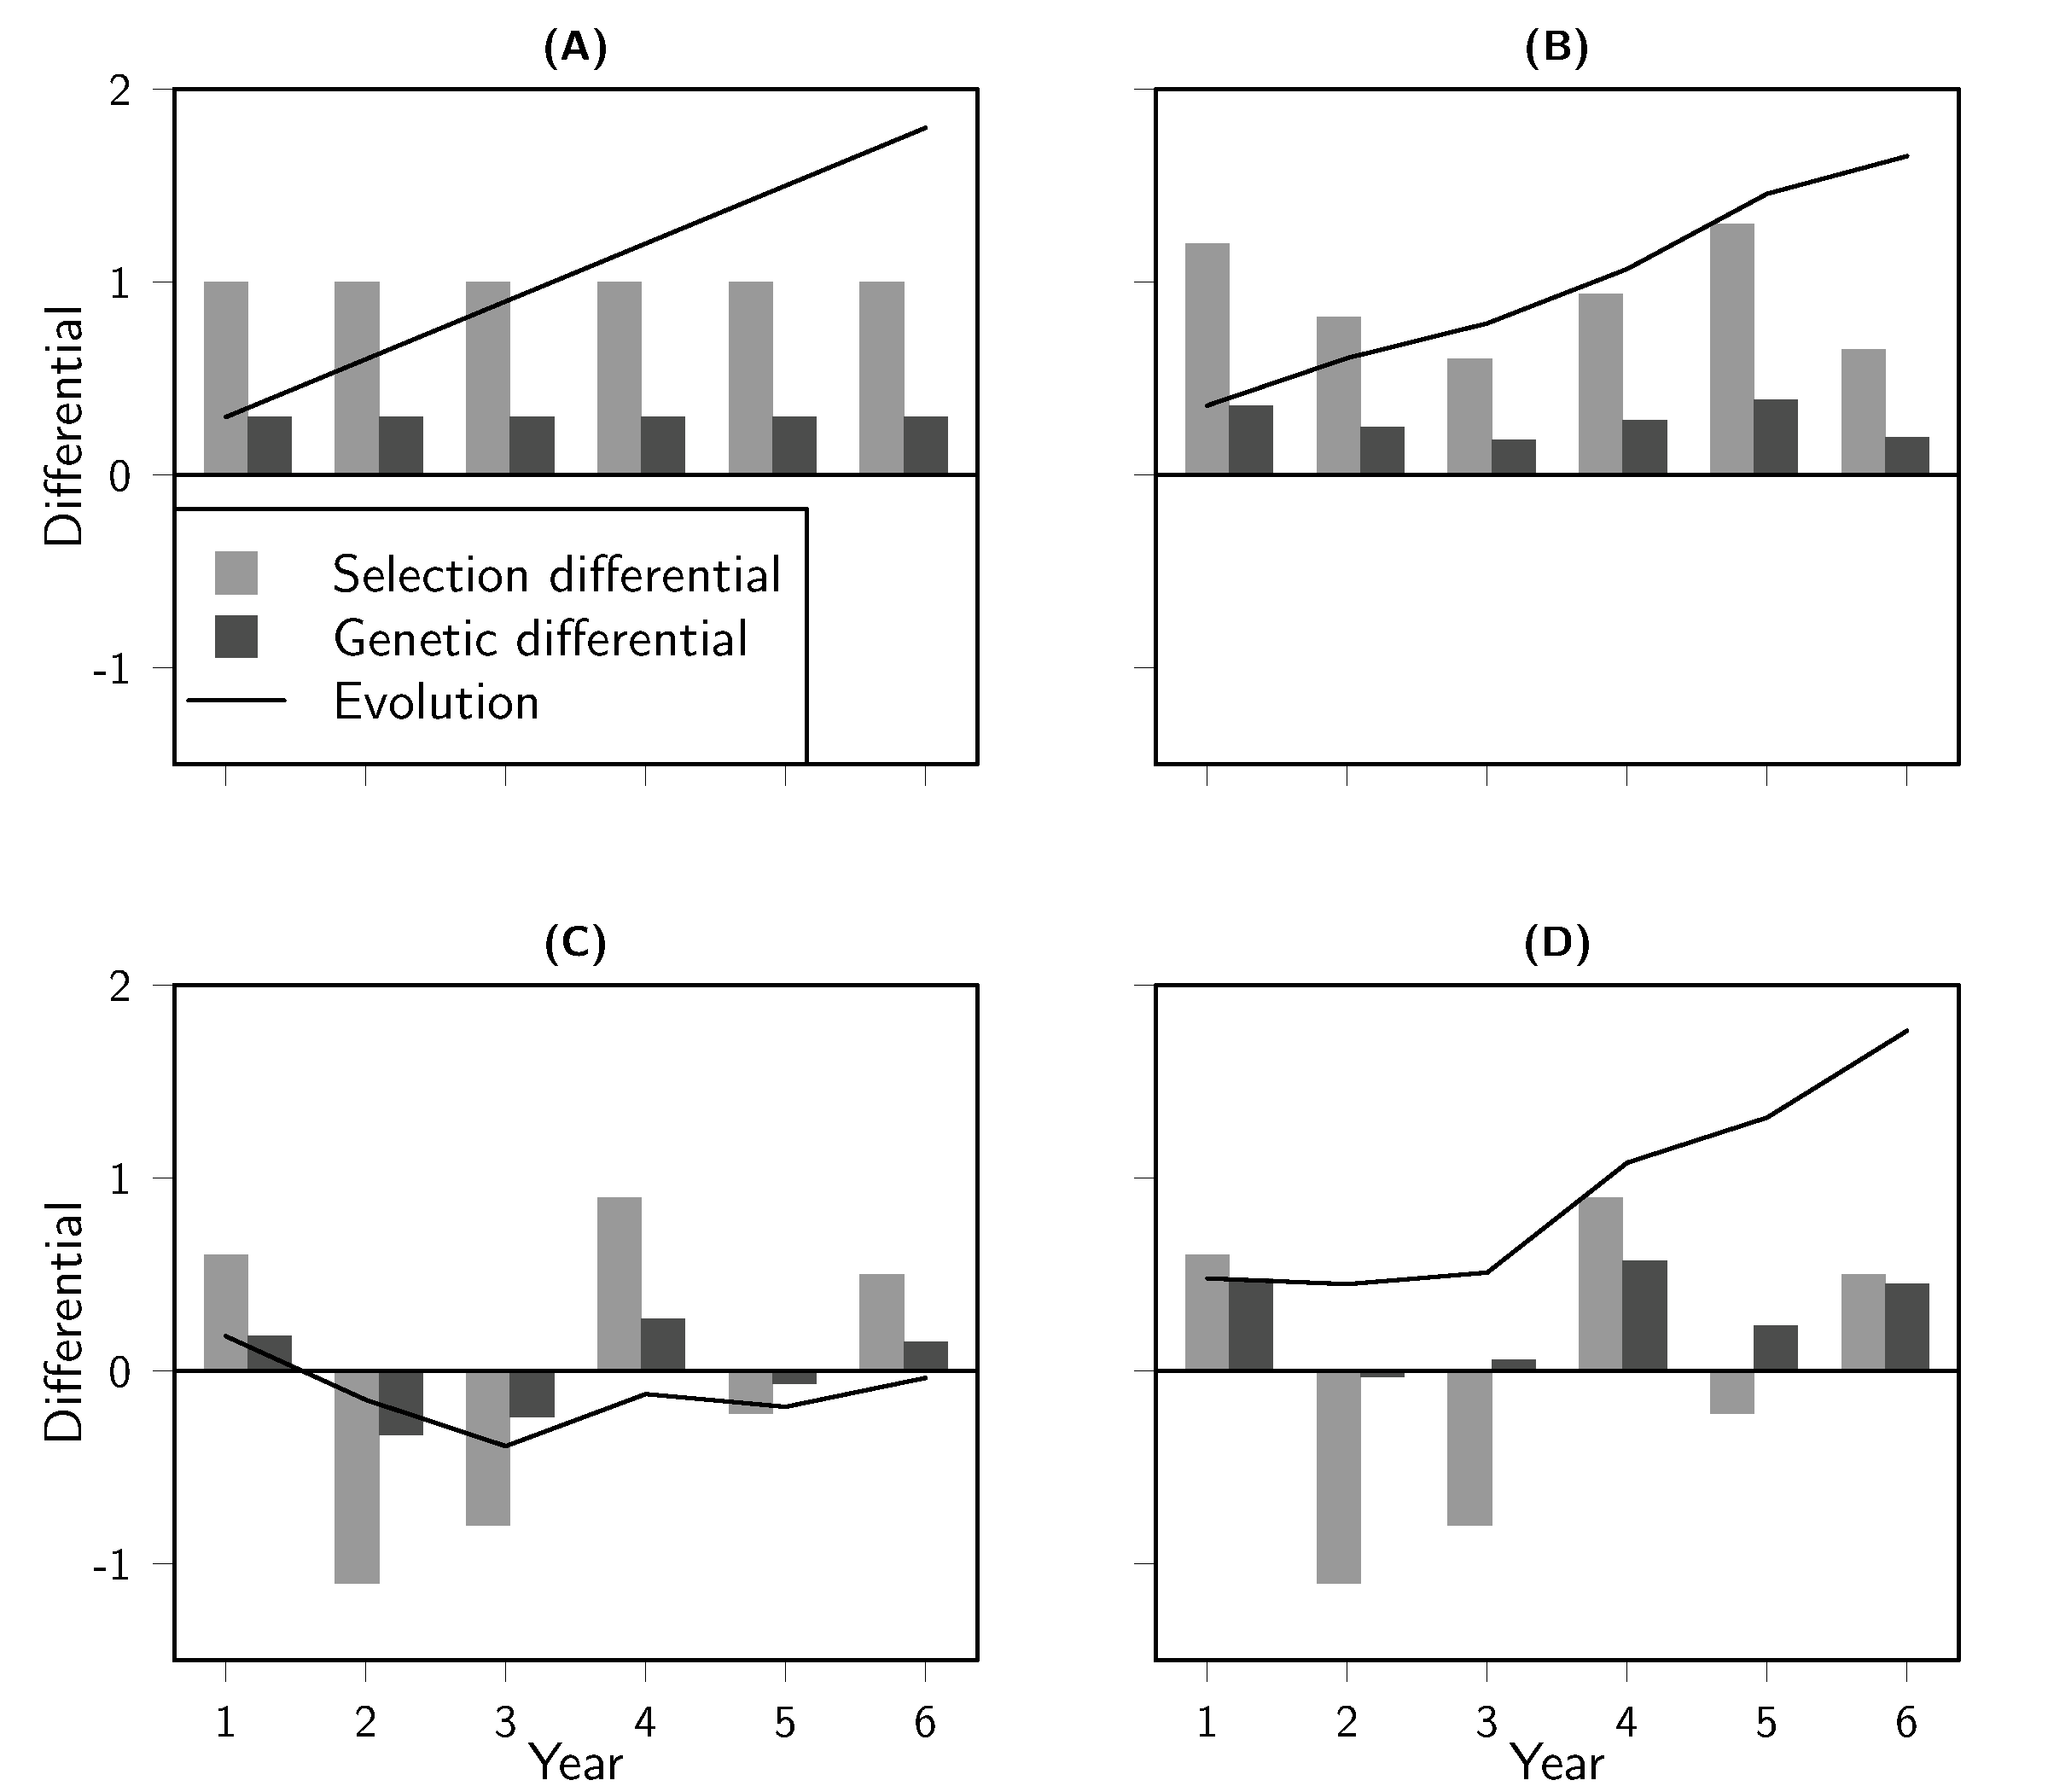
\includegraphics[width=\maxwidth]{figure/concetpualplot-1} 

\end{knitrout}

\end{document}
